% Nama Kelompok : Kelompok 3
% Kelas : D4 TI 1A
% 1. Kadek Diva Krishna Murti (1174006)
% 2. Niko
% 3. Rizal Rony Sitorus
% 4. Jeremia
% 5. Sri Rahayu (1174015)

\section{Pengertian Bit Parity}
Bit Parity merupakan bit tambahan yang disisipkan pada urutan bit-bit data yang ditransmisikan.
Tujuan pemberian bit parity ini adalah untuk memastikan bahwa bit - bit yang ditransmisikan tidak mengalami perubahan nilai setelah sampai di penerima.
Perubahan nilai dapat terjadi karena pengaruh noise atau sinyal liar.
Perubahan nilai : 0 $\,\to\,$ 1 atau 1 $\,\to\,$ 0
\newline Contoh :
\begin{table}[h!]
\centering
\begin{tabular}{ c c c }
0110100 & $\,\to\,$ &  0100100\\
\hline
Tx &  & Rx \\
\end{tabular}
\end{table}

\begin{figure}[ht]
\centerline{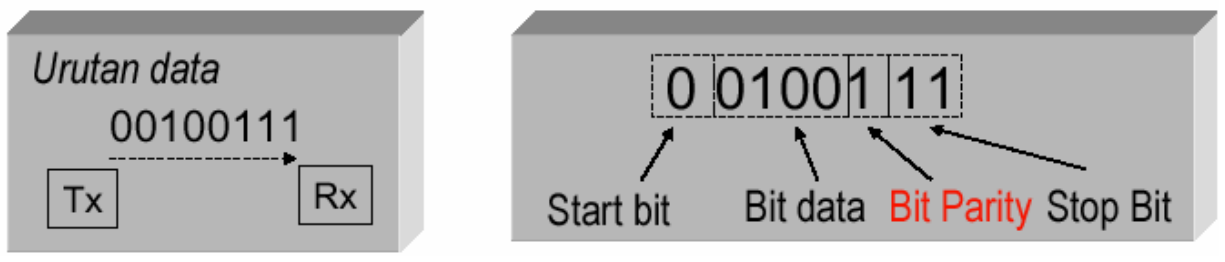
\includegraphics[width=1\textwidth]{figures/perubahan_nilai_bit_parity.png}}
\caption{Contoh perubahan nilai pada bit parity.}
\label{perubahan_nilai_bit_parity}
\end{figure}

Proses perubahan nilainya bisa dilihat pada gambar \ref{perubahan_nilai_bit_parity}

